\newcommand{\basedir}{fablab-document}
\documentclass{\basedir/fablab-document}

\usepackage{minitoc} % Inhaltsübersicht je Section
% \usepackage{fancybox} %ovale Boxen für Knöpfe - nicht mehr benötigt
\usepackage{amssymb} % Symbole für Knöpfe
% \usepackage{subfigure,caption}
\usepackage{eurosym}
\usepackage{tabularx} % Tabellen mit bestimmtem Breitenverhältnis der Spalten
\usepackage{wrapfig} % Textumlauf um Bilder
\usepackage{todonotes}

\renewcommand{\texteuro}{\euro}

\linespread{1.2}

\date{Oktober 2015}
\author{}
\title{Einweisung Kreissäge}

\begin{document}
 % Hinweise an Package minitoc, doch bitte irgendwas zu generieren - wird für späteres \secttoc benötigt
\dosecttoc
\faketableofcontents
\mtcsettitle{secttoc}{Arbeitsschritte}
\mtcsettitlefont{secttoc}{\large \sffamily \bfseries}
\mtcsetfont{secttoc}{subsection}{\sffamily}
% \mtcset
% hier geht das eigentliche Dokument los

\color{red}
\hrule
\begin{center}
\large{Achtung! Einweisung ist noch in Arbeit!}
\vspace{0.1cm}
\end{center}
\hrule
\color{black}

\section[Allgemeine Sicherheitshinweise]{Allgemeine Sicherheitshinweise}
\begin{itemize}
\item Hände bei aktiver Säge immer vom Sägebereich und dem Sägeblatt fernhalten. Die Kreissäge immer mit beiden Händen halten, entweder am Zusatzgriff oder dem Motorgehäuse. Wenn beide Hände die Kreissäge halten, kann das Sägeblatt diese nicht verletzen.

\item Nicht unter das Werkstück greifen. Die Schutzhaube kann unterhalb des Werkstückes nicht vor dem Sägeblatt schützen.

\item Die Schnitttiefe an die Dicke des Werkstücks anpassen. Es sollte weniger als eine volle Zahnhöhe unter dem Werkstück sichtbar sein.

\item Das zu sägende Werkstück niemals in der Hand oder über dem Bein halten. Das Werkstück stabil und sicher fixieren. Es ist wichtig, das Werkstück gut zu befestigen,
um die Gefahr von Körperkontakt, Klemmen des Sägeblattes oder Verlust der Kontrolle zu minimieren.

\item Auf keinen Fall so sägen, dass das Stromkabel getroffen werden kann. Die Metallteile des Elektrowerkzeugs könnten sonst unter Spannung stehen und einen elektrischen Schlag verursachen.

\item Beim Schneiden immer einen Anschlag oder eine gerade Kantenführung verwenden. Dies verbessert die Schnittgenauigkeit und verringert die Möglichkeit, dass das Sägeblatt klemmt.

\item Nur Sägeblätter in der richtigen Größe und mit passender Aufnahmebohrung (z.B. sternförmig oder rund) verwenden. Sägeblätter, die nicht zu den Montageteilen der Säge passen, laufen unrund und führen zum Verlust der Kontrolle oder beschädigen die Säge.

\item Niemals beschädigte oder falsche Sägeblatt-Spannflansche oder -Schrauben verwenden. Die Sägeblatt-Spannflansche und Schrauben wurden speziell für diese Säge konstruiert, für optimale Leistung und Betriebssicherheit.

\item Im Arbeitsbereich dürfen sich keine Unbeteiligten befinden
\end{itemize}


\section{Schutzausrüstung}

\begin{itemize}
\item Gehörschutz
\item Schutzbrille
\item Staubmaske bei stauberzeugenden Arbeiten 
\item Schutzhandschuhe beim Bearbeiten rauher Materialien und beim Werkzeugwechsel.
\end{itemize}

\section{Bestimmungsgemäße Verwendung}
Tauchsägen sind bestimmungsgemäß zum Sägen von Holz, holzähnlichen Werkstoffen, gips- und zementgebundenen Faserstoffen sowie Kunststoffen vorgesehen. Mit den von Festool angebotenen Spezialsägeblättern für Aluminium können die Maschinen auch zum Sägen von Aluminium verwendet werden. Es dürfen nur Sägeblätter mit folgenden Daten verwendet werden
\begin{itemize}
\item Sägeblattdurchmesser 160 mm;
\item Schnittbreite 2,2 mm; Aufnahmebohrung 20 mm;
\item Stammblattdicke max. 1,8 mm; geeignet für Drehzahlen bis 9500 min-1. Keine Schleifscheiben einsetzen.
\item Die Kreissäge darf ausschließlich von eingewiesene Personen verwendet werden.
\item Für die Verwendung der Kreissäge im Arbeitstisch ist eine gesonderte Einweisung erforderlich.
\end{itemize}

\subsection{Aluminiumbearbeitung}
Bei der Bearbeitung von Aluminium sind aus Sicherheitsgründen folgende besonderen Maßnahmen einzuhalten:
\begin{itemize}
\item Maschine an ein geeignetes Absauggerät anschließen.
\item Maschine regelmäßig von Staubablagerungen im Motorgehäuse reinigen.
\item Nur Aluminium-Sägeblätter verwenden.
\item Sichtfenste/ den Spanflugschutz schließen.
\end{itemize}


\section{Inbetriebnahme}
Maschine vor dem Anschließen und Lösen der Netzanschlussleitung stets ausschalten! Anschließen und Lösen der Netzanschlussleitung siehe Bild [2].
Schieben Sie die Einschaltsperre nach oben und drücken Sie den Ein-/Ausschalter (drücken= Ein / loslassen = AUS).
Die Betätigung der Einschaltsperre entriegelt die Eintauchvorrichtung. Das Sägeaggregat kann nach unten bewegt werden. Dabei taucht das Sägeblatt aus der Schutzhaube aus.

\section{Einstellungen}
\subsection{Funktionen der Maschine}
\begin{itemize}
\item Sanftanlauf: Der elektronisch geregelte Sanftanlauf sorgt für ruckfreien Anlauf des Elektrowerkzeugs.
\item Konstante Drehzahl: Die Motordrehzahl wird elektronisch konstant gehalten. Dadurch wird auch bei Belastung eine gleichbleibende Schnittgeschwindigkeit erreicht.
\item Drehzahlregelung: Die Drehzahl lässt sich mit dem Stellrad stufenlos einstellen. Dadurch können die Schnittgeschwindigkeit der jeweiligen Oberfläche optimal angepasst werden 
\item Temperatursicherung: Bei zu hoher Motortemperatur werden Stromzufuhr und Drehzahl reduziert. Die Maschine läuft nur noch mit verringerter Leistung, um eine rasche Abkühlung durch die Motorlüftung zu ermöglichen. Wenn die Übertemperatur andauert, schaltet die Maschine nach ca. 40 sec komplett ab. Erst nach Abkühlung des Motors ist ein erneutes Einschalten möglich.
\item Strombegrenzung: Die Strombegrenzung verhindert bei extremer Überlastung eine zu hohe Stromaufnahme. Dies kann zu einer Verringerung der Motordrehzahl führen. Nach Entlastung läuft der Motor sofort wieder an.
\item Bremse: Die TS 55 REBQ besitzt eine elektronische Bremse. Nach dem Ausschalten wird das Sägeblatt in ca. 2 Sekunden elektronisch zum Stillstand abgebremst.
\end{itemize}

\subsection{Schnitttiefe einstellen}
Die Schnitttiefe lässt sich von 0 - 55 mm am Schnitttiefenanschlag einstellen. Das Sägeaggregat kann nun bis zur eingestellten Schnitttiefe nach unten gedrückt werden. 
\begin{itemize}
\item Schnitttiefe ohne Führungsschiene: max. 55 mm
\item Schnitttiefe mit Führungsschiene FS: max. 51 mm
\end{itemize}

\subsection{Schnittwinkel einstellen}
TODO siehe Anleitung

\subsubsection{Sägeblatt wechseln}
TODO siehe Anleitung

\section{Arbeiten mit der Maschine}
TODO siehe Anleitung

\section{Zeichnungen}
\begin{figure}[h]
	\centering
%	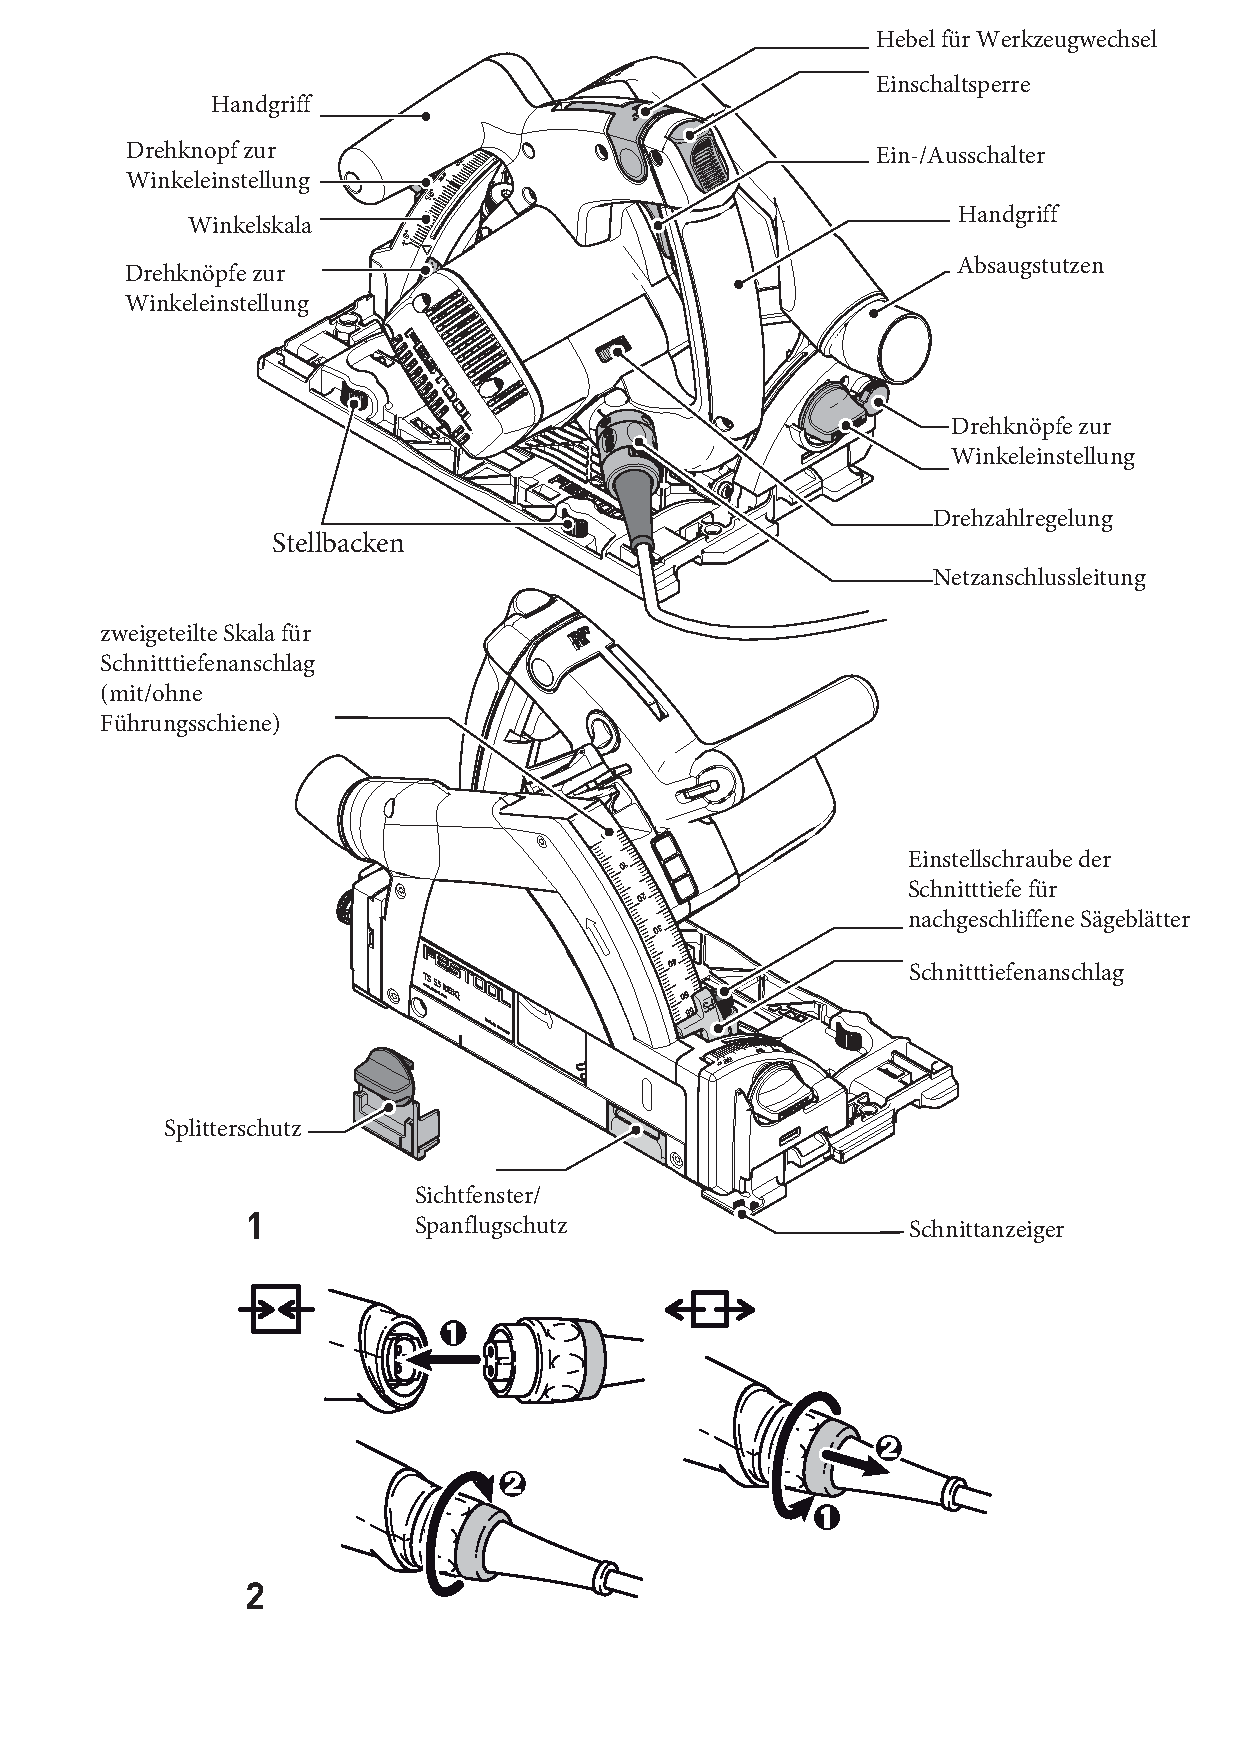
\includegraphics[width=1\textwidth]{img/festool_bilder_1Teil1.pdf}
	\caption{}
	\label{fig:gehaeuse_oben}
\end{figure}

\begin{figure}[h]
	\centering
%	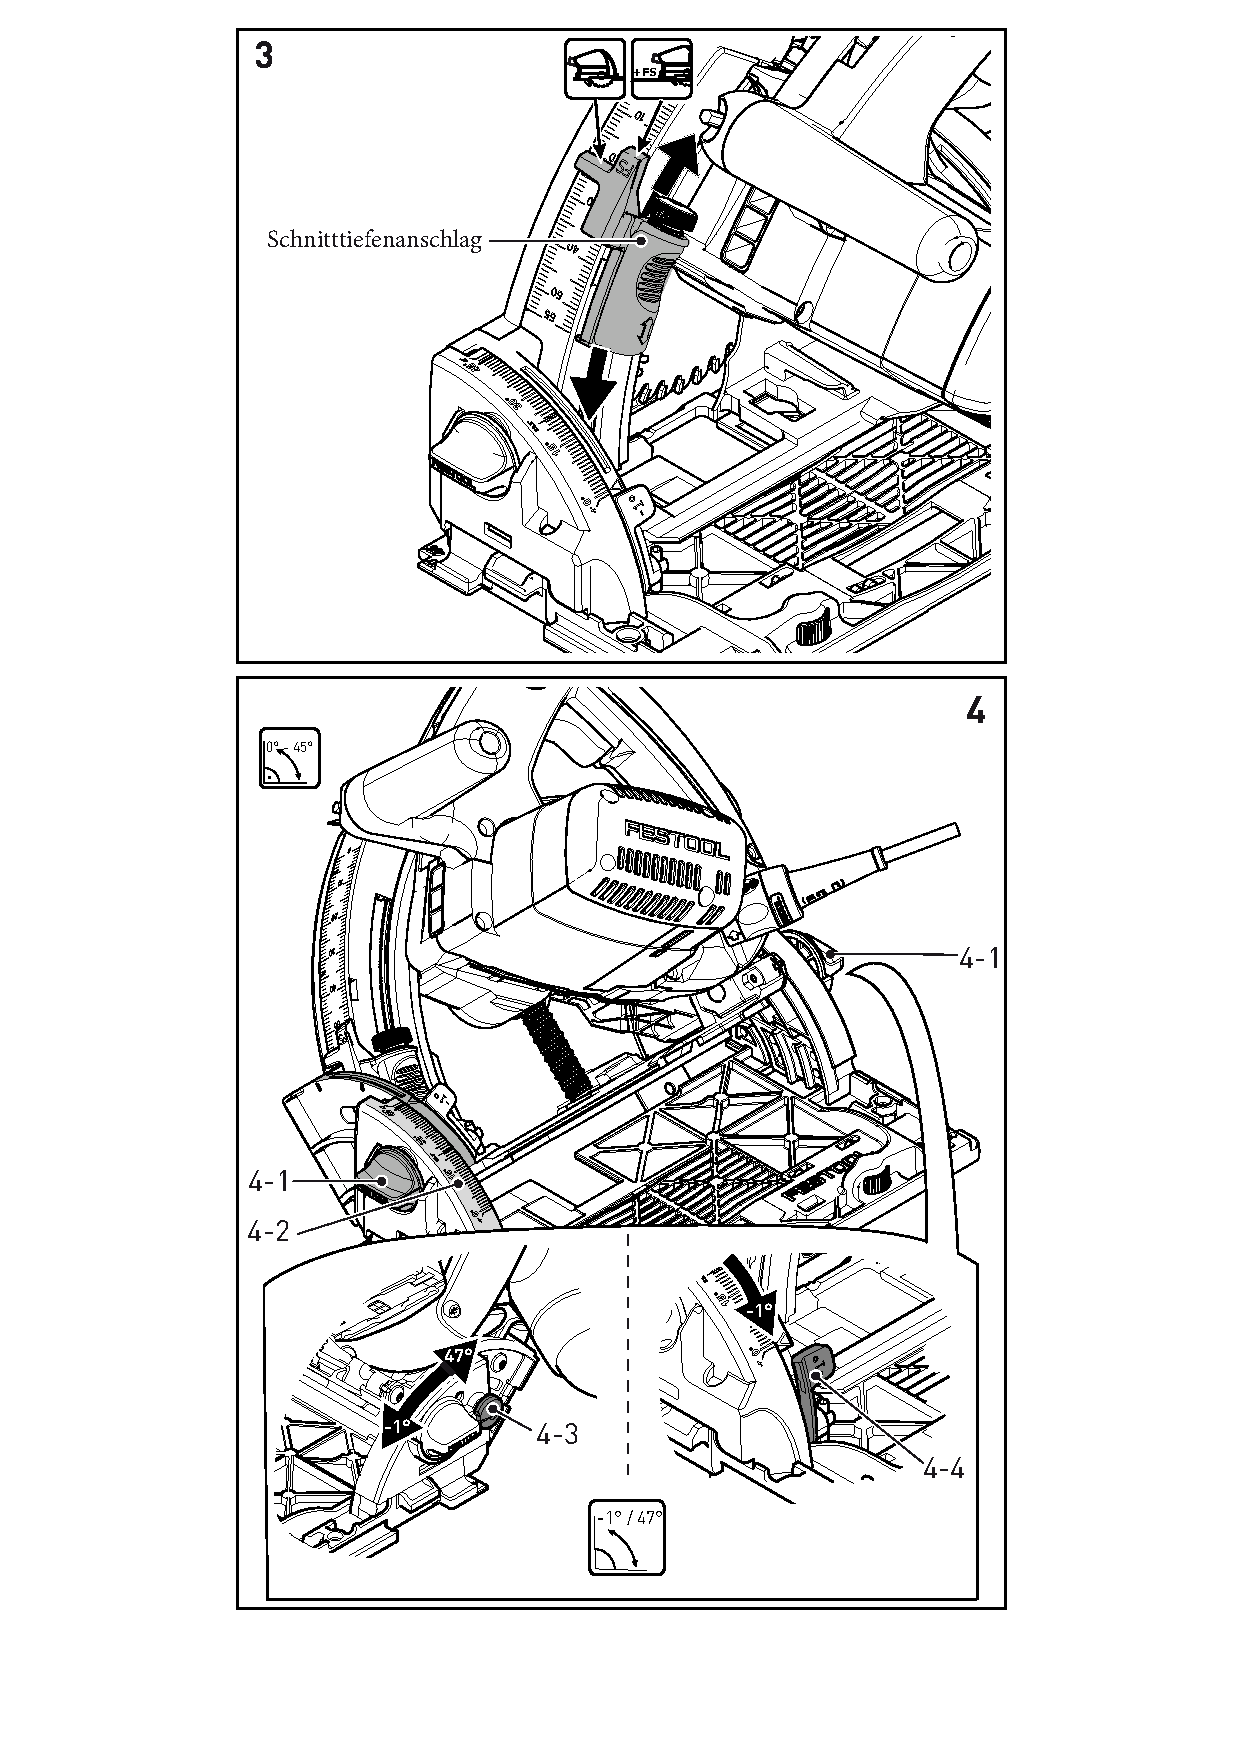
\includegraphics[width=1\textwidth]{img/festool_bilder_1Teil2.pdf}
	\caption{}
	\label{fig:gehaeuse_oben}
\end{figure}

\begin{figure}[h]
	\centering
%	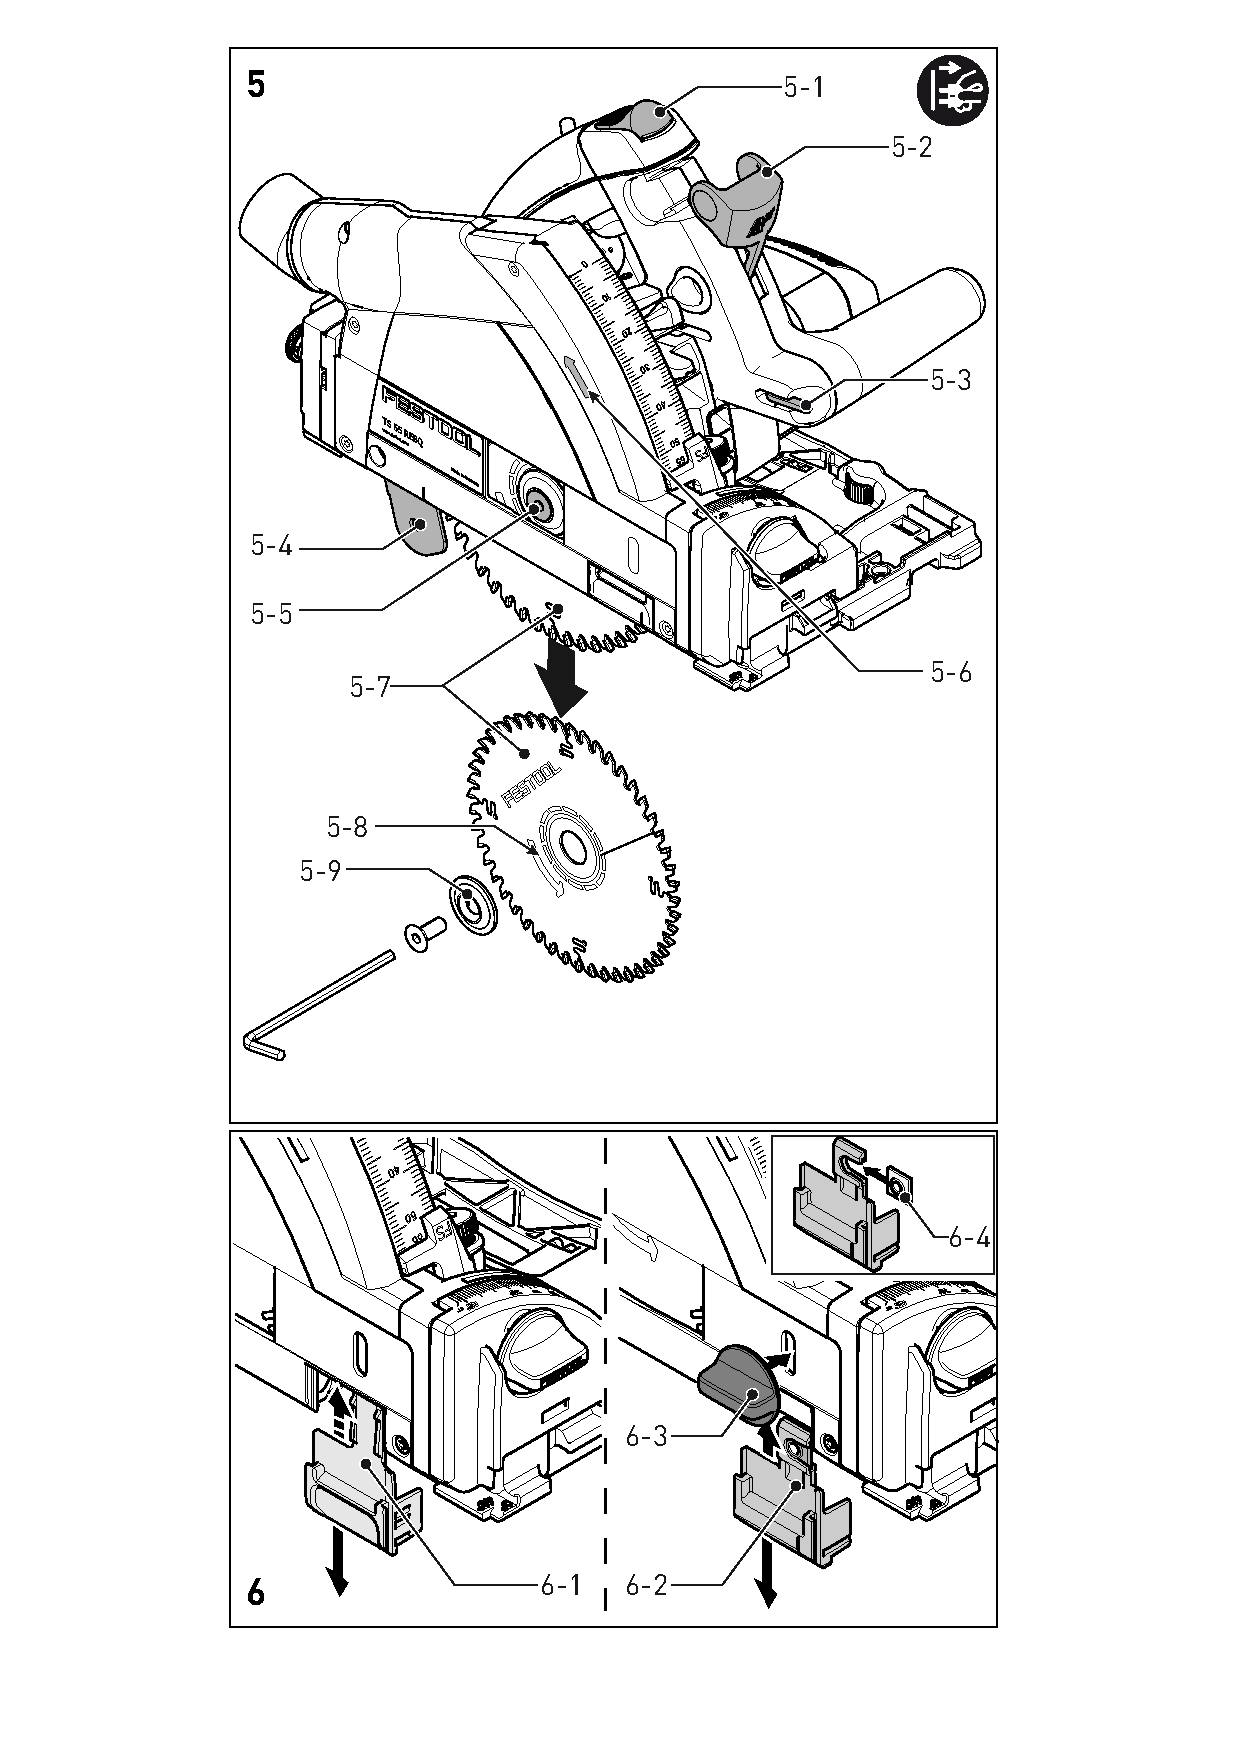
\includegraphics[width=1\textwidth]{img/festool_bilder_2Teil1.pdf}
	\caption{}
	\label{fig:gehaeuse_oben}
\end{figure}

\begin{figure}[h]
	\centering
%	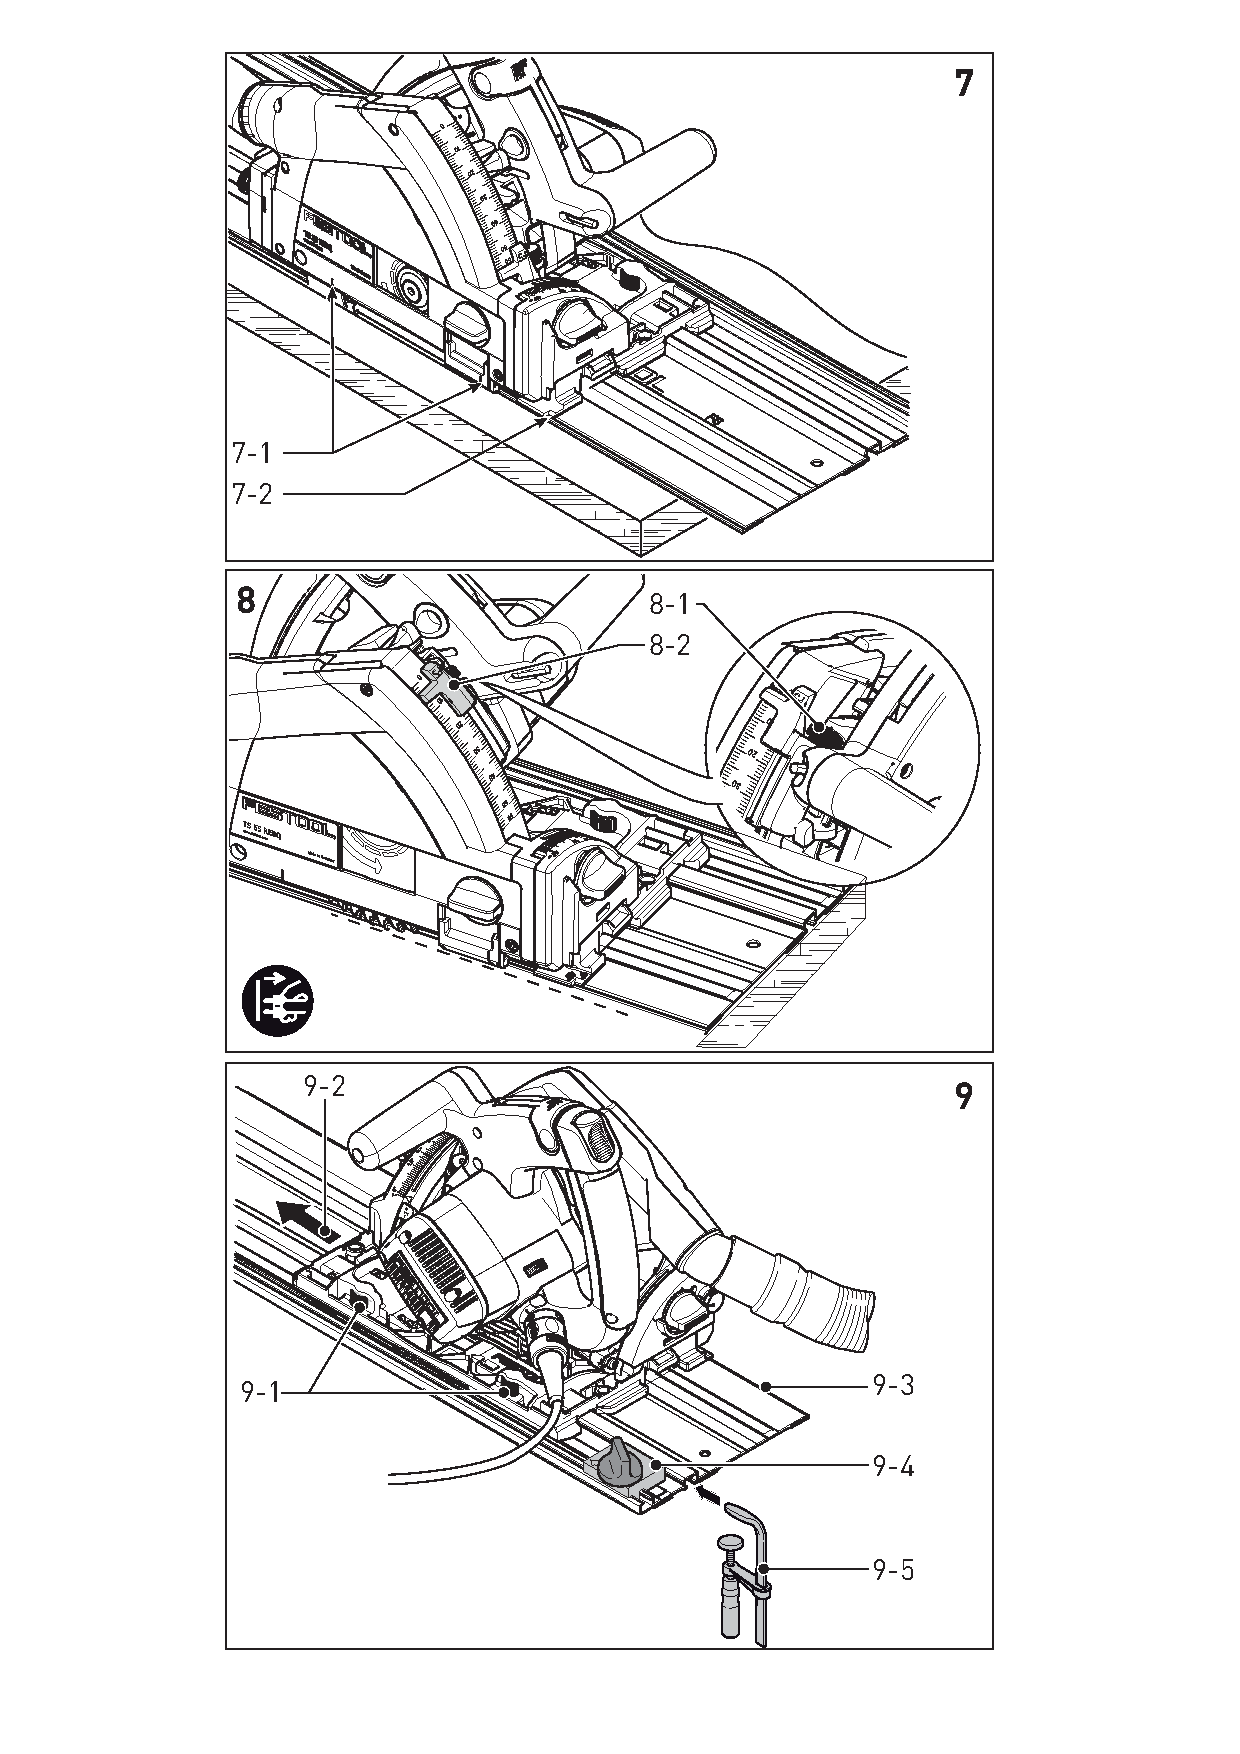
\includegraphics[width=1\textwidth]{img/festool_bilder_2Teil2.pdf}
	\caption{}
	\label{fig:gehaeuse_oben}
\end{figure}


\newpage
\section{Quellen}
\begin{itemize}
\item Festool \glqq Originalbetriebsanleitung\grqq TS 55 REBQ unter 
\url{http://www.etracker.de/lnkcnt.php?et=6hsNGE&url=https\%3a\%2f\%2fassets.festool.com\%2fmedia\%2f706758_002_ts55rebq.zip&lnkname=Bedienungsanleitung+TS+55}
\end{itemize}

\end{document}
